\documentclass[10pt,letterpaper]{article}
\usepackage[utf8]{inputenc}
\title{EV 2.4 GIRO DE UN MOTOR DE CORRIENTE DIRECTA}
\author{Ascencio De Leon Agustin}
\usepackage[spanish]{babel}
\usepackage{graphicx}
\graphicspath{{IMG/}}
\usepackage[left=2.5cm,top=2.5cm,bottom=3cm,right=2.5cm]{geometry}


\begin{document}
\maketitle
\begin{figure}
\centering 
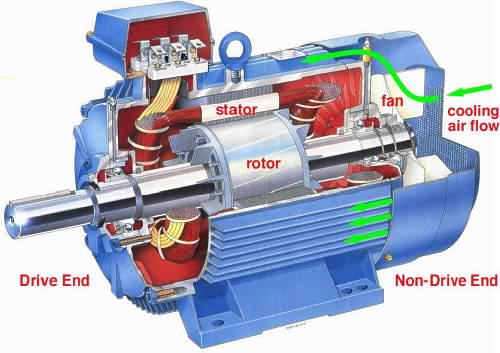
\includegraphics[scale=.5]{01}
\end{figure}
\newpage

\section{Introducción}
Los motores eléctricos de corriente continua son el tema de base que se amplia en el siguiente trabajo, definiéndose en el mismo los temas de más relevancia para el caso de los motores eléctricos de corriente continua, como lo son: su definición, los tipos que existen, su utilidad, distintas partes que los componen, clasificación por excitación, la velocidad, la caja de bornes y otros mas.

Esta máquina de corriente continua es una de las más versátiles en la industria. Su fácil control de posición, par y velocidad la han convertido en una de las mejores opciones en aplicaciones de control y automatización de procesos. Pero con la llegada de la electrónica su uso ha disminuido en gran medida, pues los motores de corriente alterna, del tipo asíncrono, pueden ser controlados de igual forma a precios más accesibles para el consumidor medio de la industria. A pesar de esto los motores de corriente continua se siguen utilizando en muchas aplicaciones de potencia (trenes y 
tranvías) o de precisión (máquinas, micro motores, etc.)

\section{Motor de corriente continua}
Un motor eléctrico de Corriente Continua es esencialmente una máquina que convierte energía eléctrica en movimiento o trabajo mecánico, a través de medios electromagnéticos.

\section{FUNDAMENTOS DE OPERACIÓN DE LOS MOTORES ELÉCTRICOS}
En magnetismo se conoce la existencia de dos polos: polo norte (N) y polo sur (S), que son las regiones donde se concentran las líneas de fuerza de un imán. Un motor para funcionar se vale de las fuerzas de atracción y repulsión que existen entre los polos. De acuerdo con esto, todo motor tiene que estar formado con polos alternados entre el estator y el rotor, ya que los polos magnéticos iguales se repelen, y polos magnéticos diferentes se atraen, produciendo así el movimiento de rotación.
Un motor eléctrico opera primordialmente en base a dos principios: El de inducción, descubierto por Michael Faraday en 1831; que señala, que si un conductor se mueve a través de un campo magnético o está situado en las proximidades de otro conductor por el que circula una corriente de intensidad variable, se induce una corriente eléctrica en el primer conductor. Y el principio que André Ampére observo en 1820, en el que establece: que si una corriente pasa a través de un conductor situado en el interior de un campo magnético, éste ejerce una fuerza mecánica o f.e.m. (fuerza electromotriz), sobre el conductor.

El movimiento giratorio de los motores de C.C. se basa en el empuje derivado de la repulsión y atracción entre polos magnéticos. Creando campos constantes convenientemente orientados en estator y rotor, se origina un par de fuerzas que obliga a que la armadura (también le llamamos así al rotor) gire buscando "como loca" la posición de equilibrio.
Gracias a un juego de conexiones entre unos conductores estáticos, llamados escobillas, y las bobinas que lleva el rotor, los campos magnéticos que produce la armadura cambian a medida que ésta gira, para que el par de fuerzas que la mueve se mantenga siempre vivo.


\section{Utilización de los motores de corriente directa C.D o corriente continua C.C}
Se utilizan en casos en los que es importante el poder regular continuamente la velocidad del motor, además, se utilizan en aquellos casos en los que es imprescindible utilizar corriente directa, como es el caso de motores accionados por pilas o baterías. Este tipo de motores debe de tener en el rotor y el estator el mismo numero de polos y el mismo numero de carbones.

\section{LOS MOTORES DE CORRIENTE DIRECTA PUEDEN SER DE TRES TIPOS:}
SERIE
\linebreak
PARALELO
\linebreak
COMPOUND
\linebreak
\section{MOTOR SERIE:}
 es un tipo de motor eléctrico de corriente continua en el cual el devanado de campo (campo magnético principal) se conecta en serie con la armadura. Este devanado está hecho con un alambre grueso porque tendrá que soportar la corriente total de la armadura.

Debido a esto se produce un flujo magnético proporcional a la corriente de armadura (carga del motor). Cuando el motor tiene mucha carga, el campo de serie produce un campo magnético mucho mayor, lo cual permite un esfuerzo de torsión mucho mayor. Sin embargo, la velocidad de giro varía dependiendo del tipo de carga que se tenga (sin carga o con carga completa). Estos motores desarrollan un par de arranque muy elevado y pueden acelerar cargas pesadas rápidamente.


\end{document}